% Template for ICASSP-2013 paper; to be used with:
%          spconf.sty  - ICASSP/ICIP LaTeX style file, and
%          IEEEbib.bst - IEEE bibliography style file.
% --------------------------------------------------------------------------
\documentclass{article}
\usepackage{spconf,amsmath,graphicx}
\usepackage{multirow}
% Example definitions.
% --------------------
\def\x{{\mathbf x}}
\def\L{{\cal L}}

% Title.
% ------
\title{AUTHOR GUIDELINES FOR ICASSP 2014 PROCEEDINGS MANUSCRIPTS}
%
% Single address.
% ---------------
\name{Author(s) Name(s)\thanks{Thanks to XYZ agency for funding.}}
\address{Author Affiliation(s)}
%
% For example:
% ------------
%\address{School\\
%   Department\\
%   Address}
%
% Two addresses (uncomment and modify for two-address case).
% ----------------------------------------------------------
%\twoauthors
%  {A. Author-one, B. Author-two\sthanks{Thanks to XYZ agency for funding.}}
%   {School A-B\\
%   Department A-B\\
%   Address A-B}
%  {C. Author-three, D. Author-four\sthanks{The fourth author performed the work
%   while at ...}}
%   {School C-D\\
%   Department C-D\\
%   Address C-D}
%
\begin{document}
%\ninept
%
\maketitle
%
\begin{abstract}
\end{abstract}
%
\begin{keywords}
Deep Neural Networks, Bottleneck feature
\end{keywords}
%
\section{Introduction}
\label{sec:intro}

\section{Model Description}

\subsection{Low-rank matrix factorization}
\begin{figure*}[htb]
  \centering
  \centerline{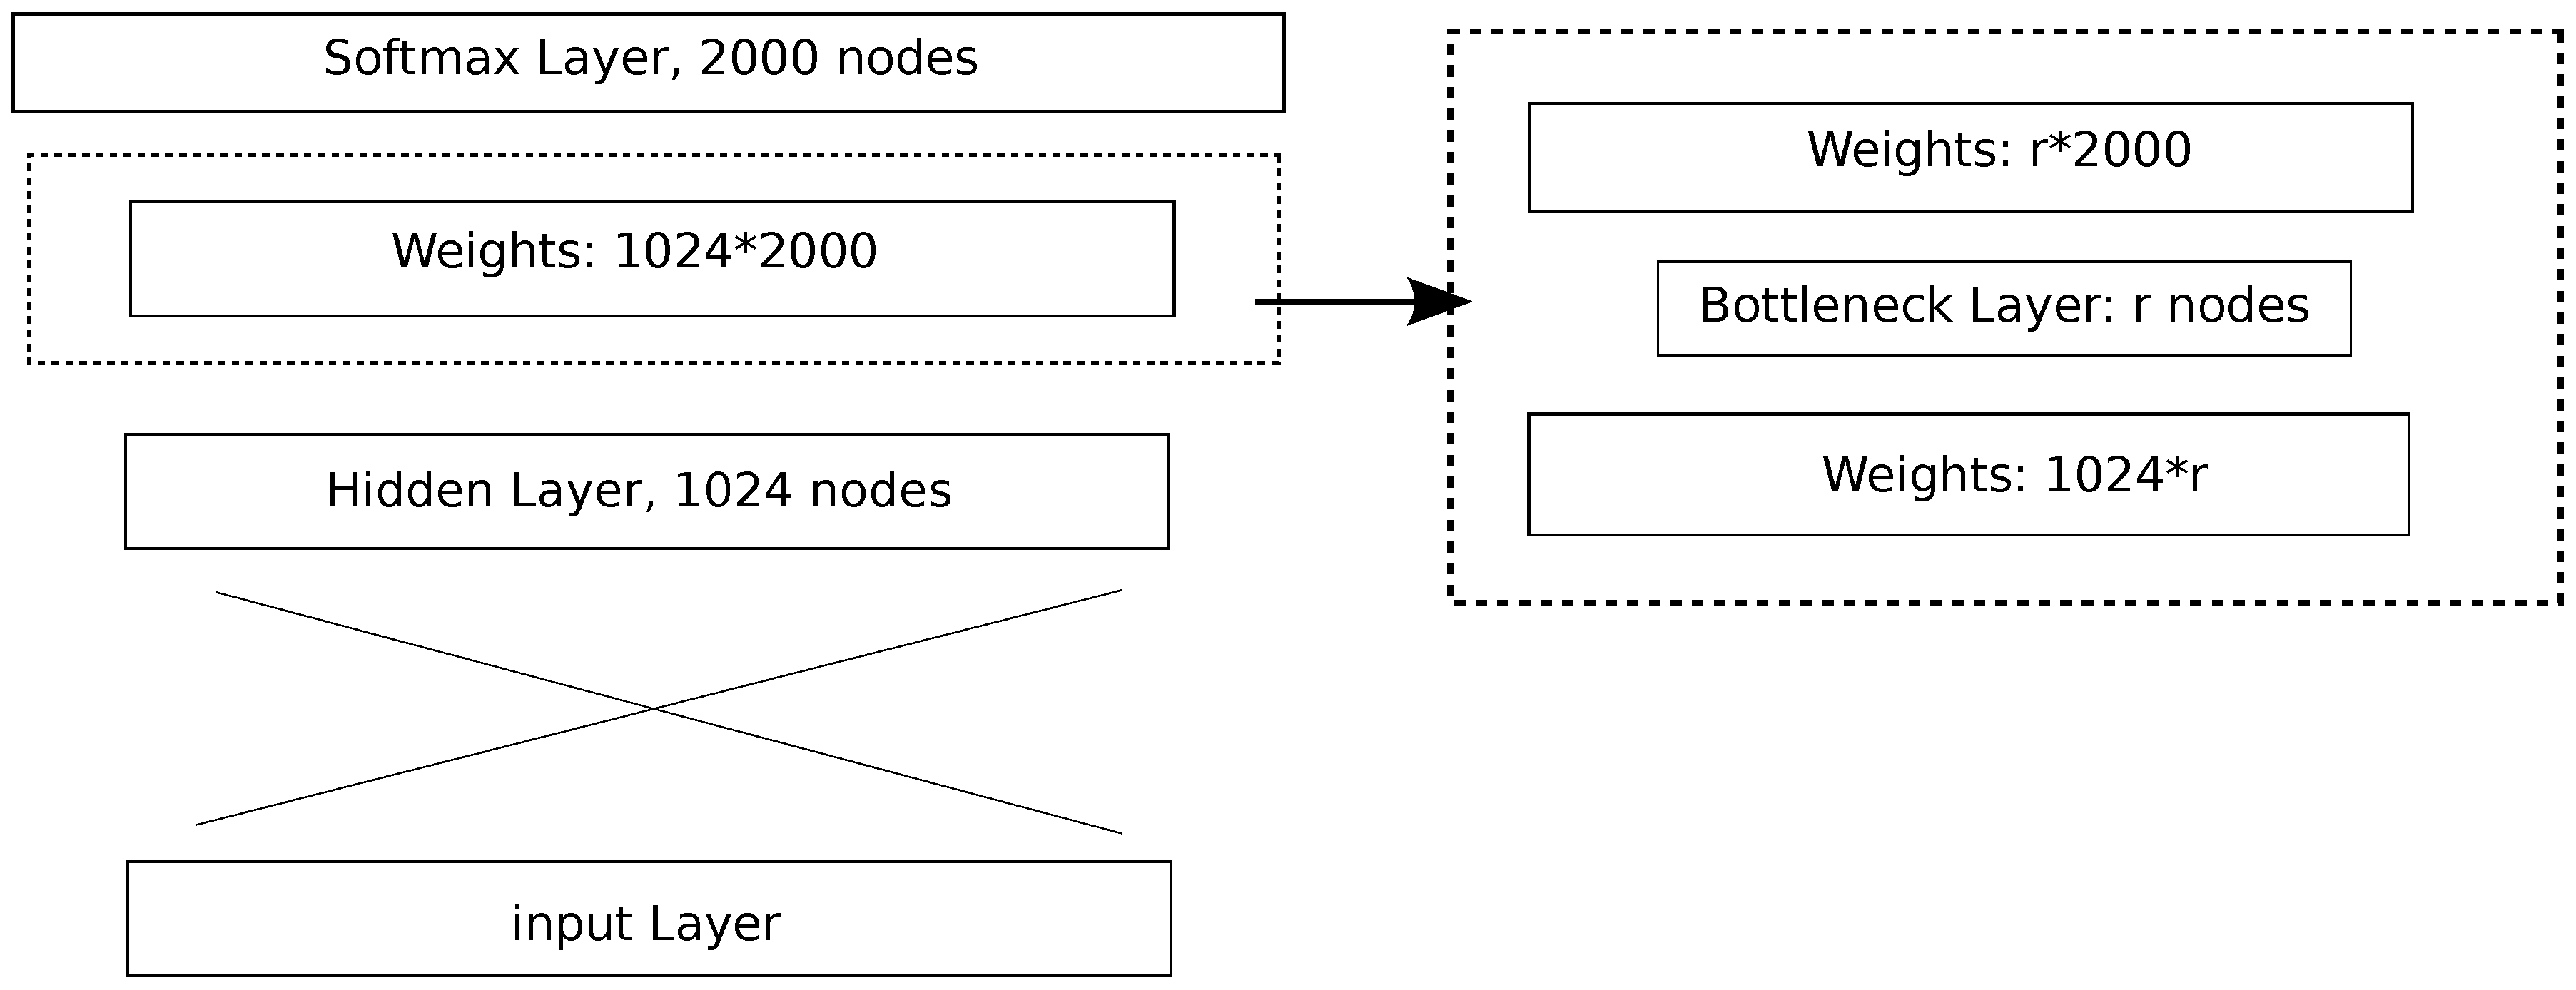
\includegraphics[width=0.8\textwidth]{lrDNN.eps}}
  \caption{Diagram of Low-rank factorized Deep Neural Network}
  \label{ref:lrDNN}
\end{figure*}

The left side of Figure \ref{ref:lrDNN} shows a typical deep neural network architecture for speech recognition problems. Following Sainath {\it{et al.}} \cite{Tara2013} we investigate a low-rank approximation to the final layer of the network, replacing it by a linear layer with a small number of hidden units followed by a softmax layer as the right side of Figure \ref{ref:lrDNN}. More specifically, inserting a new bottleneck output layer with $r$ linear hidden units to the last
weight matrix with a hidden layer of size $h$ and a softmax layer with $s$ state posterior outputs. It changes the parameters from $h*s$ to $r*(h+s$. Notice there is no non-linearity for this bottleneck outputs layer. The benefit of this structure is twofold. First, this method ensures that the best achievable frame accuracy when given a relative small size layer (as in \cite{Tara2013}). Secondly, the linearity of the output for the bottleneck layer imply that we could model
these DNN extracted features directly through a simple logistic regression and achieve a good classification results.

\subsection{Stacked Bottleneck features}
\begin{figure*}[htb]
  \centering
  \centerline{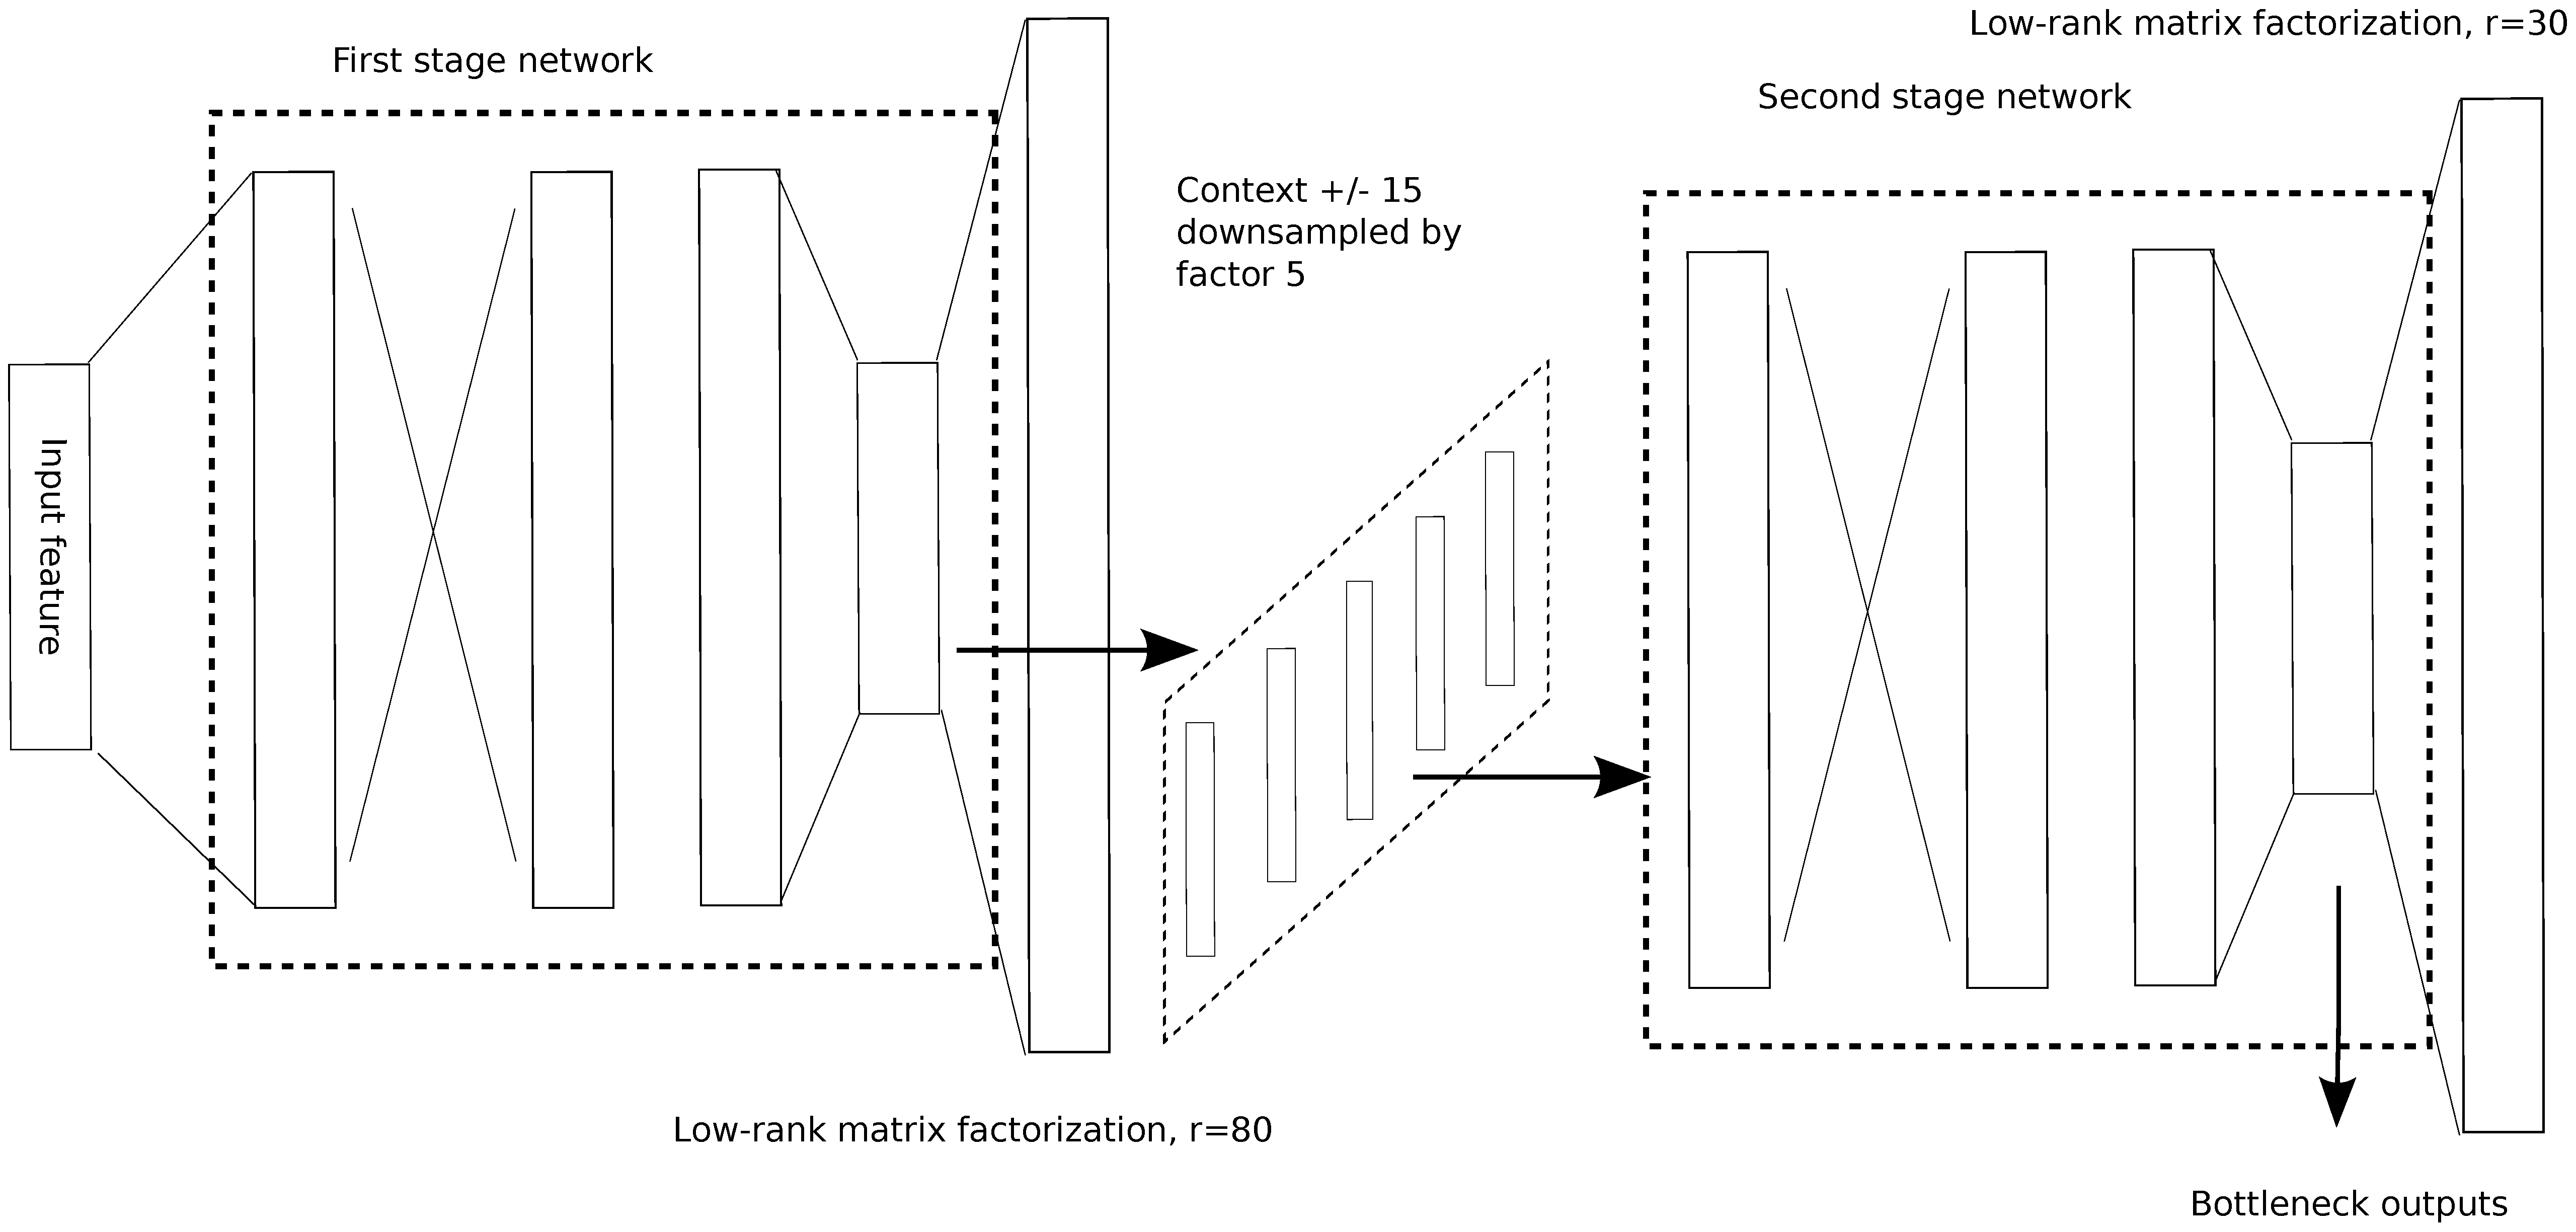
\includegraphics[width=0.8\textwidth]{stackNN.eps}}
  \caption{Diagram of stacked bottleneck neural network feature extraction}
  \label{ref:stackDNN}
\end{figure*}

Stacked Bottleneck features has shown the power in babel project \cite{Martin2013}. In our system, we follow this structure except we use the tied-states as the outputs targets and place all the BN layer in the last hidden layer. In \cite{Tara2013} has shown that the hidden layers do not have the same low-rank properties, so in our system, we place all the BN layer in the last hidden layer.



\begin{itemize}
  \item this low-rank technique to DNN 
\end{itemize}

\section{System description}
\subsection{Data}
The BABEL data simulate a case of what one could collect in limited time from a completely new language: it consists of two parts: scripted (speaker read text through telephone channel) and conversational (spontaneous telephone conversations). The test data contains conversational speech only. In our experiments, we only use the conversational part for training.

For turkish, the phoneme set consists of \dots

\subsection{Baseline HMM system}
\label{baseline}
Baseline HMM system setup and evaluation of trained model were done using Kaldi recognition tookit \cite{Kaldi}. 

For feature extraction in front-end, we use 13 PLP features which concatenated with F0 estimates and the probability of voicing (the implementation of F0 and probability of voicing estimation followed \cite{F0}). Conversational-side based mean and variance normalization was applied was applied in both training and recognition stages. For acoustic modeling, we used phonetic decision based tied-state triphone CDHMMs with around 2500 states (depend on the languages) and 18 Gaussian components per state. Final word transcriptions are decoded using 3gram Language Model (LM) trained only on the transcriptions of training
data\footnote{This is coherent to BABEL rules, where the provided data only can be used for system training in the primary condition.}.

After extracting the plp features, we build-up the baseline system as follows:
\begin{itemize}
  \item The resulting 15-dimentional features are concatenated $\pm 4$ frames to produce $135$ dimensional vectors.
  \item Then LDA is used to reduce the dimensionality to $40$ which considers HMM states as classes. 
  \item Applying MLLT \cite{MLLT} as a feature orthogonalizing transform that makes the features more accurately modeled by diagonal-covariance Gaussians.
  \item Global fMLLR \cite{fmllr} is applied to normalize inter-speaker variability (for both training and test).
\end{itemize}

\subsection{DNN training setup}
The DNN system setup were also done using Kaldi recognition tookit \cite{Kaldi}. The neural networks had 6 hidden layers. The output layer is a softmax layer, and the outputs represent the log-posterior of the output labels, which correspond to context-dependent HMM states (there are around 2500 states depends on different languages). The network input are the speaker adapted feature from the baseline case (both for training and test) and concatenated with $\pm 5$ frames (the
total size is $40*11=440$). The number of nodes for each hidden layers are the same which contain 1024 hidden units. The nonlinearities in the hidden layers are sigmoid fnuctions and the objective function is the cross-entropy criterion. The alignment of context-dependent states to frames derives from the GMM baseline systems and left fixed during training.

The DNN is pretrained by Restricted Boltzmann Machines \cite{RBM} and fune-tune using ``new-bob'' algorithm. The initialization of the network and the learning rate we followed \cite{kaldiDNN}. Both of the pretraining and fune-tune was done on GPUs using \cite{Kaldi}.

\subsection{LrSBNs for feature extraction}

The input features of the first NN (Figure \ref{ref:stackDNN}) are 23 Critical-Band Energies obtained with a Mel filter-bank, with conversation-side-based mean subtraction applied. 11 frames of these features are stacked with a Hamming window multiplies the time evolution of each parameter and DCT is applied, of which 0th to 5th coefficients are retained\cite{Martin2013}. Finally, the pitch and voicing feature are concatenated, making the size of the feature vector
$(23+2)*6 = 150$.

The input features of the second NN are the outputs the bottleneck layer from the first NN. Context expansion by concatenation of frames with time offsets $-10,-5,0,5,10$. The overall time context is $31$ frames. Both NNs has the same 5 hidden sigmoid layer and 1 linear layer and were trained to classify tied-states. There targets were generated by forced alignment from the baseline models (section \ref{baseline}).

The final BN features produced by the stacked NN were do a PCA transform and then using this feature vector, a context-dependent system was trained starting from a the baseline system in section \ref{baseline}.

\section{Analysis of LrSBN features}

\subsection{The best layer of bottleneck features}
Past research \cite{Martin2013} has shown the performance is improved when putting a linear layer in the middle. However, \cite{Tara2013} has shown that the hidden layers do not have the same low-rank properties. Table  shows the cross-validation frame accuracy. We could observed that the performance of putting a linear layer in the middle even worse than the original sigmoid layer. As expected, the low-rank softmax-layer got the best frame accuracy.

\subsection{Context-independent or Context-dependent}
In \cite{Martin2013} and \cite{CMU2013}, the neural network was trained to classify phoneme states. However, we have similar observations as \cite{MSBN}, using the context-dependent targets is always better than context-independent targets. Table \ref{lab:CI} compares the performance of the BN systems using labels generated from different acoustic models. The first row in the table shows that if context-dependent labels are used, 3.2\% gain is obtained for the single neural network.
Finally, if the context-dependent labels are used for the stacked neural network, we still got improvement of 1.7\% although it relative smaller. So in the further experiments of our system, we always use context-independent labels and putting the bottleneck layer as the last hidden layer.

\begin{table}[htb]
  \centering
  \caption{Comparison of Using Context-independent or Context-dependent targets}
  \label{lab:CI}
  \begin{tabular}{|l|l|l|}
    \hline
    \multicolumn{2}{|c|}{Baseline} & 80.8\%\\
    \hline\hline
    \multirow{2}{*}{Single NN} & CI targets & 77.4\%\\
     & CD targets & 74.2\%\\ \hline
     \multirow{2}{*}{Stacked NN} & CI targets & 73.1\%\\
     & CD targets & 71.4\%\\ \hline
   \end{tabular}
\end{table}
\subsection{Low-rank on the softmax layer}
In order to determine whether the low-rank factorization on the softmax layer is necessary, we evaluated the features generated by different active layer.
We test this condition on Bengali limited language pack. In the first row of Table \ref{tab:linear}, we test feature on pure bottleneck feature directly (without any post-processing for the bottleneck outputs). In the second row, we do on PCA on top of the output feature (from 80 dim to 30 dim) and add the $\Delta$ and $\Delta^2$ feature to model the context information. It can be seen that for both condition, the LrSBN could achieve a better performance.
\begin{table}[htb]
  \centering
  \caption{Comparison of Using low-rank factorization of traditional sigmoid activation, the plp baseline is $75.3\%$}
  \label{tab:linear}
  \begin{tabular}{|l|l|l|l|}
    \hline
      & SBN & LrSBN\\\hline
    raw BN & 70.8\% & 69.2\%\\\hline
    raw BN (pca) + $\Delta$ + $\Delta^2$ & 68.1\% & 67.2\%\\\hline
  \end{tabular}
\end{table}

\subsection{Results on Larger task and different languages}
Further evaluation of the proposed architecture was done on the different language and using a speaker-adapted model. On this task, we compared with the GMM-HMM system, Hybrid system and the BN system we proposed. The top of Table \ref{tab:limited} shows that with standard ML training, an improvement of over $10\%$ relative could be achieved when using LrSBNs which even better than a hybrid DNN system (using the speaker-adapted feature as the input), lowering the WER from $68.0\%$ to
$67.2\%$. With speaker-adaptation training and MPE discriminative training, the relative gain is still high around $8.0\%$ relative. Similar results were obtained on the Assamese dataset on the below of Table \ref{tab:limited}.
\begin{table}[htb]
  \centering
  \caption{Results on Bengali and Assamese Limited system (10 h)}
  \label{tab:limited}
  \begin{tabular}{|l|c|c|c|}
    \hline
    AM Training & ML & LDA+MLLT & SAT+MPE \\\hline\hline
    \multicolumn{4}{|c|}{Bengali}\\\hline
    plp+F0 & 75.3\% & 74.4\% & 71.8\% \\\hline
    DNN & * & * & 68.0\%\\\hline
    BN+$\Delta$+$\Delta$ & 67.2\% & * & 66.1\% \\\hline\hline
    \multicolumn{4}{|c|}{Assamese}\\\hline
    plp+F0 & 74.6\% & 73.0\% & 70.5\% \\\hline
    DNN & & & 67.2\%\\\hline
    BN+$\Delta$+$\Delta$ & 65.8\% & * & 65.1\% \\\hline\hline
  \end{tabular}
\end{table}

Now that we have studied the behavior on a limited condition. We also explore the behavior of the LrSBN features on larger 100 hours Bengali full condition task. The comparison of recognition performance is given in Table \ref{tab:full}. It can be seen the relative gain even larger then the limited condition, $12.6\%$ relative gain, lowering the WER from $64.5\%$ to $56.4\%$. It is also better than the Hybrid DNN system, improving the performance from $59.4\%$ to $56.4$.
\begin{table}[htb]
  \centering
  \caption{Results on Bengali full system (100 h)}
  \label{tab:full}
  \begin{tabular}{|l|c|c|c|}
    \hline
    AM Training & ML & LDA+MLLT & SAT+MPE \\\hline\hline
    \multicolumn{4}{|c|}{Bengali full}\\\hline
    plp+F0 & 69.2\% & 68.4\% & 64.5\% \\\hline
    DNN & * &* & 59.4\%\\\hline
    BN+$\Delta$+$\Delta$ & 59.6\% & * & 56.4\% \\\hline\hline
  \end{tabular}
\end{table}

\subsection{Discussion}

\section{Conclusion}


\section{REFERENCES}
\label{sec:refs}

% References should be produced using the bibtex program from suitable
% BiBTeX files (here: strings, refs, manuals). The IEEEbib.bst bibliography
% style file from IEEE produces unsorted bibliography list.
% -------------------------------------------------------------------------
\bibliographystyle{IEEEbib}
\bibliography{refs}

\end{document}
